\section{แนวคิดและวิธีการดำเนินงาน}

งานวิจัยนี้นำเสนอแนวทางในการสร้างกรณีทดสอบและข้อมูลทดสอบสำหรับ{\TestPath} โดยการรวบรวม{\StaticInformation}
เพื่อประกอบการพิจารณา โดยกรณีทดสอบที่สร้างขึ้นสามารถทดสอบเส้นทางการเรียกหากันระหว่าง{\class}อย่างน้อย 
1 เส้นทาง ซึ่งภาพรวมการดำเนินงานวิจัยนั้นเป็นดังรูปที่ \figpageref{fig:methodologyoverview} ซึ่งอธิบายได้ดังนี้

\begin{sidewaysfigure}
    \centering
    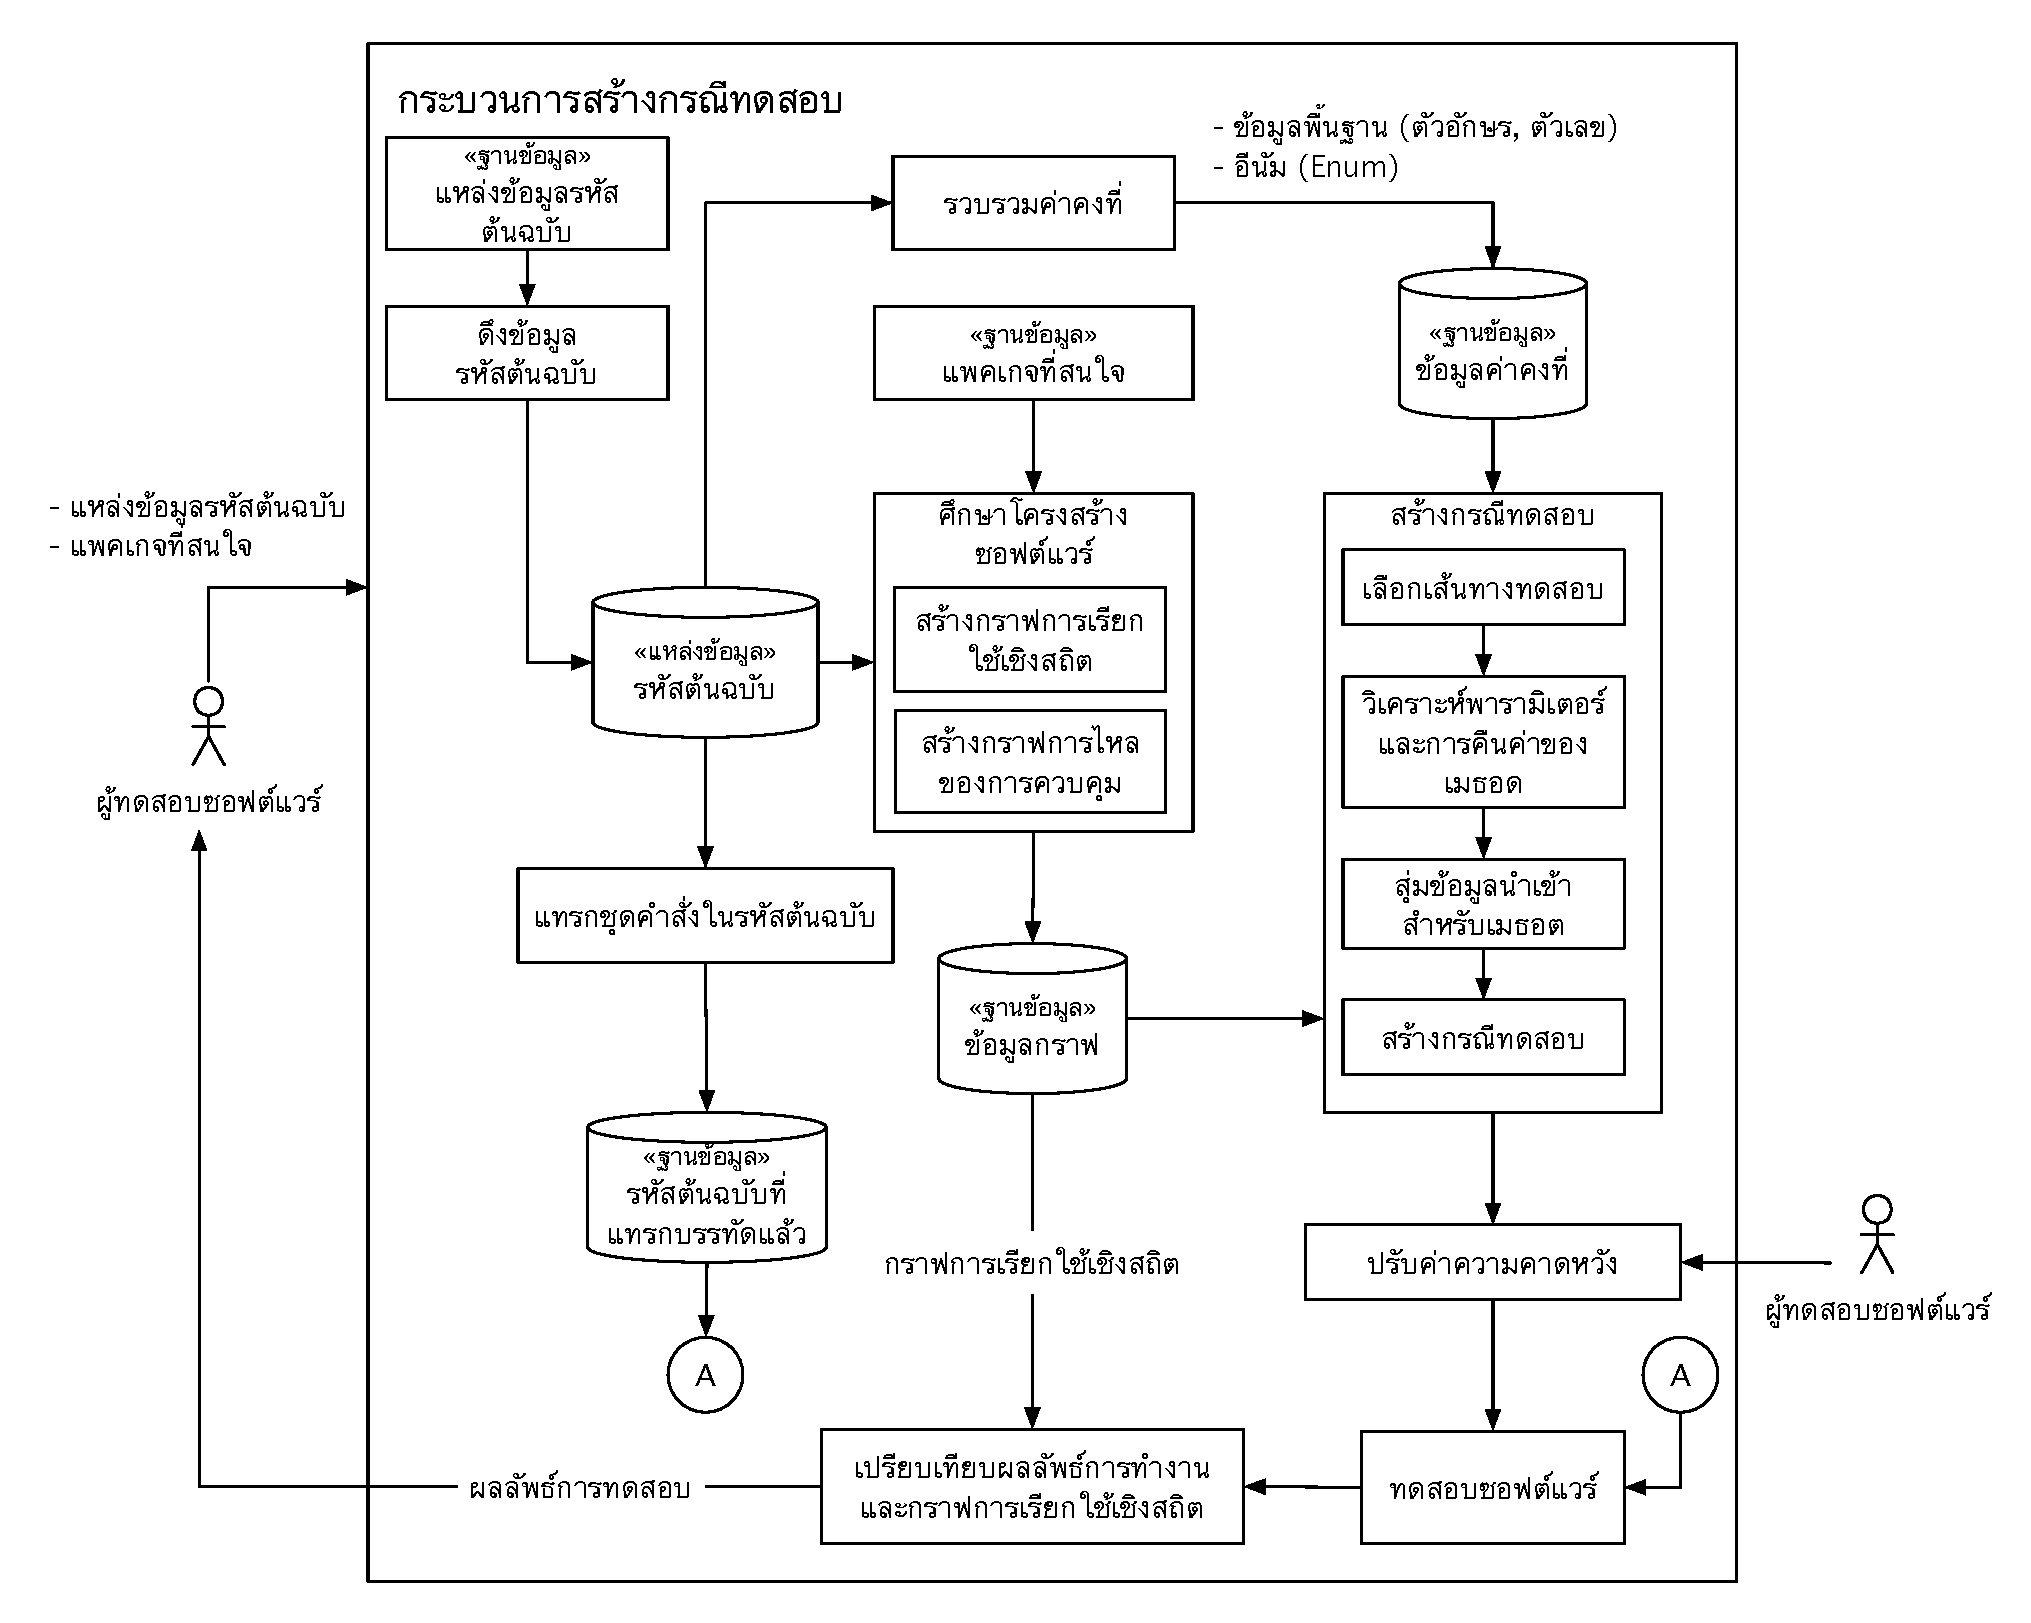
\includegraphics[width=0.9\textwidth]{methodology-overview}
    \caption{ภาพรวมการดำเนินงานวิจัย}
    \label{fig:methodologyoverview}
\end{sidewaysfigure}


\subsection{การวิเคราะห์ข้อมูลเบื้องต้น}
กระบวนการดำเนินงานนั้นจะเริ่มต้นด้วยการอ่าน{\sourcecode}จาก{\Repository}

\subsubsection{การทำเหมืองข้อมูลค่าคงที่ (2)}
\subsubsection{การสร้างกราฟ (3)}
\subsubsection{การแทรกชุดคำสั่ง (4)}

\subsection{การสร้างกรณีทดสอบ}

\begin{figure}[ht!]
    \centering
    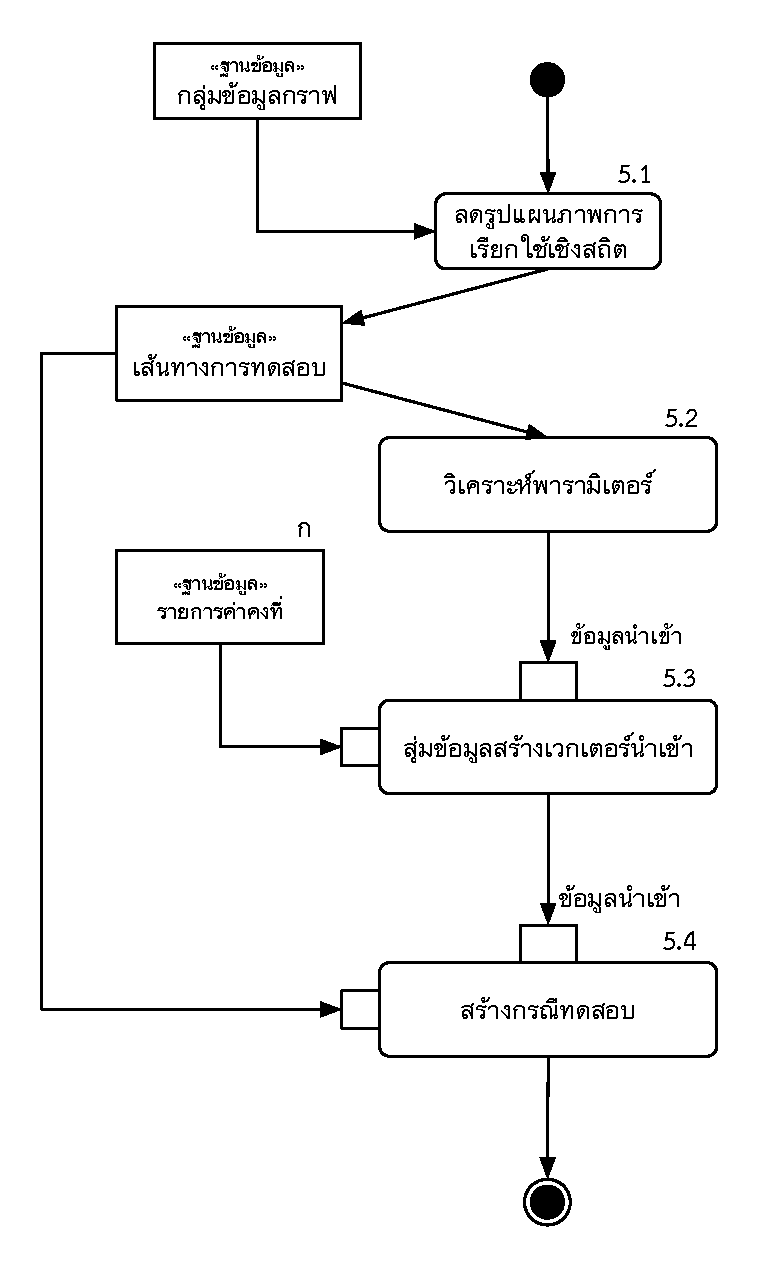
\includegraphics[width=0.5\textwidth]{methodology-activities-test-case-gen}
    % 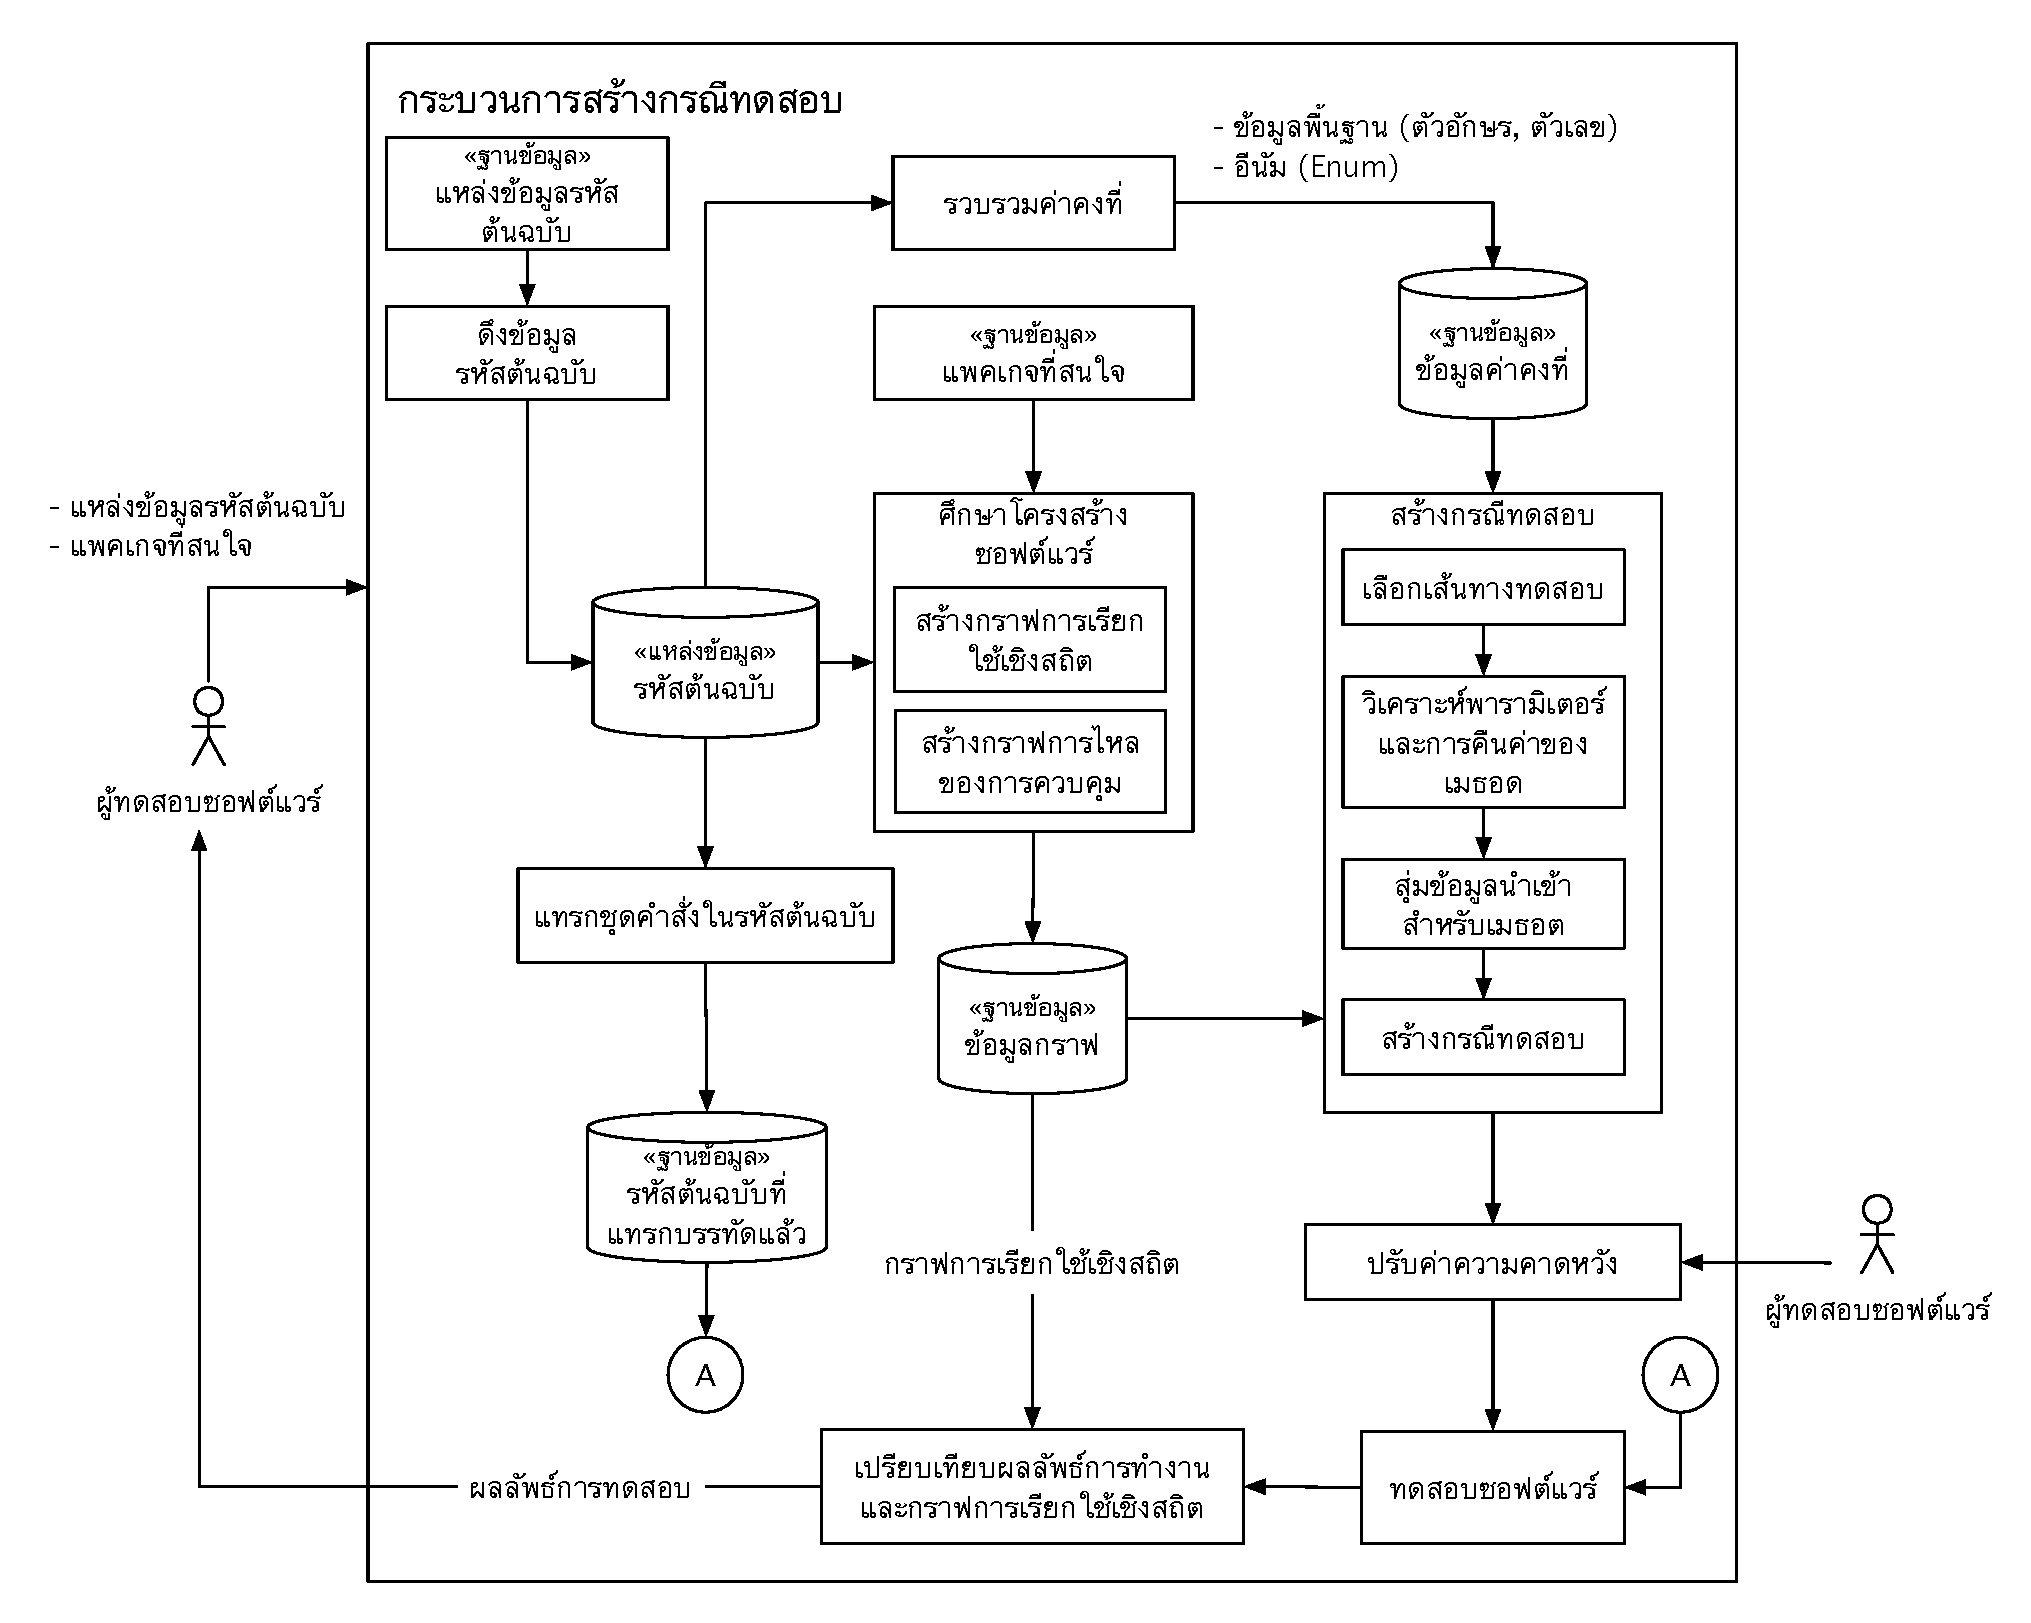
\includegraphics[width=0.9\textwidth]{methodology-overview}
    \caption{ขั้นตอนการสร้างกรณีทดสอบ}
    \label{fig:testcaseGenerationActivity}
\end{figure}

\subsubsection{เลือก\{TestPath}}
\subsubsection{การวิเคราะห์พารามิเตอร์และการคืนค่าของ{\method}}
\subsubsection{สร้างเวกเตอร์นำเข้า}
\subsubsection{สร้างกรณีทดสอบ}

\subsection{การปรับค่าความคาดหวัง}

\subsection{การทดสอบซอฟต์แวร์}

\subsection{เปรียบเทียบผลลัพธ์การดำเนินงาน}

จากรูปที่ \ref{fig:methodologyoverview} การดำเนินงานวิจััยจะเริ่มต้น
